
 \documentclass[11pt]{article}

\usepackage{graphics}
\usepackage{amsmath}
\usepackage{float}
\usepackage[margin=1in]{geometry}
\usepackage{fancyhdr}
\usepackage{authblk}

\providecommand{\keywords}[1]{\textbf{\textit{Keywords: }} #1}

\title{Power for Balanced Linear Mixed Models with Complex Missing Data Processes}
\date{\vspace{-5ex}}
\lhead{Josey et. al.}
\author[1]{Kevin P. Josey}
\author[2]{Brandy M. Ringham}
\author[1]{Anna E. Bar\a'on}
\author[3]{Margaret Schenkman}
\author[4]{Katherine A. Sauder}
\author[5]{Keith E. Muller}
\author[6]{Dana Dabelea}
\author[4,*]{Deborah H. Glueck}
\affil[1]{Department of Biostatistics and Informatics, Colorado School of Public Health, University of Colorado Denver}
\affil[2]{Lifecourse Epidemiology of Adiposity and Disease (LEAD) Center, Colorado School of Public Health, University of Colorado Denver}
\affil[3]{Physical Therapy Program, University of Colorado School of Medicine, University of Colorado Denver}
\affil[4]{Department of Pediatrics, University of Colorado School of Medicine, University of Colorado Denver}
\affil[5]{Department of Health Outcomes and Biomedical Informatics, College of Medicine, University of Florida}
\affil[6]{Department of Epidemiology and the Lifecourse Epidemiology of Adiposity and Diabetes (LEAD) Center, Colorado School of Public Health, University of Colorado Denver}
\affil[*]{Corresponding Author: Deborah H. Glueck, Deborah.Glueck@ucdenver.edu}

\begin{document}

\maketitle

\begin{abstract}
	When designing repeated measures studies, both the amount and the pattern of missing outcome data can affect power. The chance that an observation is missing may vary across measurements, and missingness may be correlated across measurements. Such complex missing data patterns affect both observational and interventional studies. For example, in a randomized trial of physiotherapy in patients with Parkinson's disease, increasing intermittent dropout over time yielded missing measurements of physical function. In this example, we assume data are missing completely at random, since the chance that a data point was missing appears to be unrelated to either outcomes or covariates. For data missing completely at random, we propose noncentral $F$ power approximations for the Wald test for balanced linear mixed models with Gaussian responses. The noncentral $F$ power approximations are based on moments of missing data summary statistics. The moments were derived assuming a conditional linear process for missingness. The approach provides approximate power for both complete-case and observed-case analyses. A complete-case analysis uses only the independent sampling units with all measurements present. An observed-case analysis uses all independent sampling units with at least one observation. Monte Carlo simulations demonstrate the accuracy of the power methods in small samples. We illustrate the utility of the method by computing power for proposed replications of the Parkinson's disease study.
\end{abstract}

\keywords{power, missing data, mixed model, multilevel, longitudinal}

\section{Introduction}
\label{intro}

In repeated measures studies, researchers observe multiple responses on a set of independent sampling units. The repeated measurements may be longitudinal (across time), spatial (across location), or multivariate (on different scales). Outcome data are missing when a measurement is not observed at a particular planned occasion. The chance that an observation is missing may vary across measurements, and missingness may be correlated across measurements. Both the amount and the pattern of missing outcome data can affect power in repeated measures studies. Such complex missing data patterns occur frequently in biomedical studies. For example, in a randomized controlled clinical trial of physiotherapy in patients with Parkinson's disease (ClinicalTrials.gov Identifier: NCT01257945) \cite{schenkman_exercise_2012}, increasing dropout over a 16 month follow-up period produced missing measurements of physical function. In this study, the chance that a data point was missing appeared to be unrelated to either outcomes or covariates.

Published power approximations use assumptions that do not match the complex missing data patterns like the one in the Parkinson's disease study. Muller \textit{et al}. \cite{muller_power_1992, muller_statistical_2007} assumed no missing data. Li and  McKeague \cite{li_power_2013} use local alternative distributions which rely on asymptotic assumptions for accuracy. Further compounding the issues with local alternatives, the use of GEE estimates has been shown to suffer from inflated Type I error rates in small samples, weakening its otherwise general appeal \cite{stiger_anova_1998}. Tu \textit{et al}. \cite{tu_power_2007} accounts for missing data in their power approximation, but they too assume local alternative distributions. Ringham \textit{et al}. \cite{ringham_multivariate_2016} accounts for missing data and uses a noncentral $F$-distribution proposed by Muller \textit{et al}. \cite{muller_power_1992, muller_statistical_2007}, but they assume that every response was independently and equally likely to be missing. 

To counteract these challenges, we provide power approximations that accommodate complex missing data processes characterized by a conditional linear model \cite{qaqish_family_2003}. We modify a noncentral $F$ power approximation for a class of mixed models with no missing data described by Muller \textit{et al}. \cite{muller_power_1992, muller_statistical_2007} and Edwards \textit{et al}. \cite{edwards_r2_2008}. The modifications incorporate the expected value of one of several missing data summary statistics. \cite{ringham_multivariate_2016, barton_hypothesis_1989, catellier_tests_2000} The choice of which missing data summary statistic to use depends on whether scientists plan \textit{complete-} or \textit{observed-}case data analytic approaches. The complete-case approach uses only independent sampling units with all measurements present. The observed-case approach uses any independent sampling unit with at least one measurement. There are two missing data summary statistics in particular that we favor for these objective analyses. 

The work applies to a broad and useful subset of missing processes, models and hypothesis tests. The data are assumed to be missing completely at random (MCAR) \cite{little_statistical_2002}. Under the MCAR assumption, the distribution of the missing responses does not depend on any of the observed outcomes, unobserved outcomes or explanatory variables. The models are assumed to be a class of general linear mixed models \cite{laird_random-effects_1982} referred to as balanced linear mixed models\cite{muller_statistical_2007, ringham_multivariate_2016}. A general linear mixed model is a balanced linear mixed model if it can be expressed as an equivalent general linear multivariate model when there is no missing data. We restrict attention to the Wald test and the Kenward-Roger reference distribution \cite{barton_hypothesis_1989, catellier_tests_2000, ringham_multivariate_2016} due to its equivalence with a Hotelling-Lawley trace test \cite{mckeon_f_1974}. We use a covariance estimator that assumes an unstructured correlation between responses which has  been shown to be quite favorable in clinical trial settings with random dropout. \cite{gosho_comparison_2017} Balanced linear mixed models fulfill the following criteria. For a particular independent sampling unit, the predictors have the same value for all outcomes. In addition, each independent sampling unit has the same number of planned predictors and the same error covariance matrix. In balanced linear mixed models with no missing data, each independent sampling unit has the same number and type of planned outcome measurements. In this manuscript, we relax the last assumption, and allow for missing data. 

The paper has six sections. Section \ref{notation} contains general notation, definitions, and model assumptions, while Section \ref{power} contains the power approximations. In Section \ref{simulations}, Monte Carlo simulations are used to demonstrate the accuracy of the method in small samples. Section \ref{illustrativeexample} contains example power analyses for a proposed clinical trial. The implications and limitations of the results are discussed in Section \ref{discussion}.

\section{Notation, Definitions, and Assumptions}
\label{notation}

\subsection{General Notation}

For an $\left(m\times o\right)$ matrix $\boldsymbol{A}$ and an $\left(o\times n\right)$ matrix $\boldsymbol{B}$, $\boldsymbol{AB}$ is the matrix product. Throughout $\text{vec}(\boldsymbol{A})$ is the matrix function that stacks the columns of an $\left(m\times n\right)$ matrix $\boldsymbol{A}$ into an $\left(mn\times 1\right)$ vector. For an $\left(m\times n\right)$ matrix $\boldsymbol{A}$ and a $\left(p\times q\right)$ matrix $\boldsymbol{B}$, the Kronecker product $\boldsymbol{A}\otimes\boldsymbol{B}$ generates the $\left(mp\times qn\right)$ matrix $\boldsymbol{C}=\left\{a_{ij}\boldsymbol{B}\right\}$. The trace of a square matrix $\boldsymbol{A}$ is $\text{tr}\left(\boldsymbol{A}\right)=\sum_{i=1}^{N}a_{ii}$. A square and full rank matrix $\boldsymbol{A}$ has inverse $\boldsymbol{A}^{-1}$. Also, for any matrix $\boldsymbol{A}$, the Moore-Penrose inverse is $\boldsymbol{A}^{+}$ and $\boldsymbol{A}'$ is the transpose. An $\left(a\times a\right)$ identity matrix is $\boldsymbol{I}_{a}$, an $\left(a\times 1\right)$ vector with every value set to $1$ is $\boldsymbol{1}_{a}$ and an $\left(a\times 1\right)$ vector with every value set to $0$ is $\boldsymbol{0}_{a}$. The minimum and maximum values of a set $\mathcal{S}$ are denoted by $\min\left\{\mathcal{S}\right\}$ and $\max\left\{\mathcal{S}\right\}$, respectively.

We indicate the expected value and variance of $\boldsymbol{y}$ as $\boldsymbol{\mathcal{E}}\left(\boldsymbol{y}\right)$ and $\boldsymbol{\mathcal{V}}\left(\boldsymbol{y}\right)$, respectively. Similarly, for scalar $y$, we indicate the expected value and variance as $\mathcal{E}\left(y\right)$ and $\mathcal{V}\left(y\right)$. Scalar random variables $y_i$ and $y_j$ have covariance $\mathcal{C}\left(y_{i},y_{j}\right)$. For positive integer $n$, we write $\boldsymbol{y}\sim N_{n}\left(\boldsymbol{\mu},\boldsymbol{\Xi}\right)$ to indicate the vector normal probability distribution \cite{arnold_theory_1981} with $\boldsymbol{\mu}\in\Re^{n}$ an $\left(n\times 1\right)$ vector of means and $\boldsymbol{\Xi}\in\left(\Re^{n}\times\Re^{n}\right)$ a positive definite symmetric $\left(n\times n\right)$ matrix of covariances. Similarly, with $N$ and $p$ positive integers, $N>p$, we write $\boldsymbol{Y}\sim N_{N,p}\left(\boldsymbol{M},\boldsymbol{\Omega},\boldsymbol{\Xi}\right)$ to indicate the matrix normal \cite{arnold_theory_1981}, with $\boldsymbol{M}\in\left(\Re^{N}\times\Re^{p}\right)$ an $\left(N\times p\right)$ matrix of means, $\boldsymbol{\Omega}\in\left(\Re^{p}\times\Re^{p}\right)$ a positive definite symmetric $\left(p\times p\right)$ matrix of column covariances and $\boldsymbol{\Xi}\in\left(\Re^{N}\times\Re^{N}\right)$ a positive definite symmetric $\left(N\times N\right)$ matrix of row covariances. Consequently, $\boldsymbol{Y}\sim N_{N,p}\left(\boldsymbol{M},\boldsymbol{I}_{N},\boldsymbol{\Xi}\right)$ implies that $\text{vec}\left(\boldsymbol{Y}\right)\sim N_{Np}\left[\text{vec}\left(\boldsymbol{M}\right),\boldsymbol{\Xi} \otimes \boldsymbol{I}_{N}\right]$.

\subsection{Balanced General Linear Mixed Model and General Linear Hypothesis}
\label{recalcitrant}

Under the assumptions in Section \ref{intro}, we define a balanced linear mixed model \cite{muller_statistical_2007, ringham_multivariate_2016}. We use the subscript $m$ to indicate mixed model components.

Independent sampling unit $i\in\left\{1,2,\ldots,N\right\}$ at measurement $j\in\left\{1,2,\ldots,p\right\}$ has response $y_{i,j}$, with $\boldsymbol{y}_{i}=\begin{bmatrix}y_{i,1}&y_{i,2}&\ldots&y_{i,p}\end{bmatrix}'$ the $\left(p\times 1\right)$ vector of responses for independent sampling unit $i$, and $\boldsymbol{y}=\begin{bmatrix}\boldsymbol{y}'_{1}&\boldsymbol{y}'_{2}&\ldots\boldsymbol{y}'_{N}\end{bmatrix}'$ the $\left(Np\times 1\right)$ vector of responses for all independent sampling units. The fixed and known $\left(N\times q\right)$ design matrix for a single outcome is $\boldsymbol{X}$, and $\boldsymbol{X}_{m}=\boldsymbol{X}\otimes\boldsymbol{I}_{p}$ is the corresponding $\left(Np\times qp\right)$ design matrix for all outcomes. The $\left(qp\times 1\right)$ vector $\boldsymbol{\beta}$ contains the unknown and constant model coefficients. In turn, $\boldsymbol{\Sigma}$ is a positive definite symmetric $\left(p\times p\right)$ covariance matrix and is the same for all independent sampling units. We define $\boldsymbol{\Psi}=\left(\boldsymbol{I}_{N}\otimes\boldsymbol{\Sigma}\right)$. Throughout, $\boldsymbol{e}\sim N_{Np}\left(\boldsymbol{0},\boldsymbol{\Psi}\right)$ is the $\left(Np\times 1\right)$ vector of errors, which implies statistical independence of $\boldsymbol{e}_{i}$ and $\boldsymbol{e}_{i'}$ for $i,i'\in\left\{1,2,\ldots,N\right\}$, $i\neq i'$. The balanced general linear mixed model is
\begin{equation}
\label{mixedmodelhuzzah}
\boldsymbol{y}=\boldsymbol{X}_{m}\boldsymbol{\beta}+\boldsymbol{e},
\end{equation}
with $\boldsymbol{y}\sim N_{Np}\left(\boldsymbol{X}_{m}\boldsymbol{\beta},\boldsymbol{\Psi}\right)$ and $\boldsymbol{y}_{i}$ independent of $\boldsymbol{y}_{i'}$ for $i,i'\in\left\{1,2,\ldots,N\right\}$, $i\neq i'$.

The $\left(a\times q\right)$ matrix $\boldsymbol{C}$ contains the between-independent-sampling-unit contrasts and the $\left(p\times b\right)$ matrix $\boldsymbol{U}$ contains the within-independent-sampling-unit contrasts. The $\left(ab\times pq\right)$ contrast $\boldsymbol{L}=\boldsymbol{C}\otimes\boldsymbol{U}'$ defines the secondary parameter $\boldsymbol{\theta}=\boldsymbol{L\beta}$ and the corresponding null hypothesis
\begin{equation}
H_0:\boldsymbol{\theta}=\boldsymbol{\theta}_{0}.
\end{equation}
The Wald parameter is defined as 
\begin{equation}
\label{zetabam}
\zeta_{W}\left(\boldsymbol{\theta},\boldsymbol{\Psi}\right)=\left(ab\right)^{-1}\left(\boldsymbol{\theta}-\boldsymbol{\theta}_{0}\right)'\left[\boldsymbol{L}\left(\boldsymbol{X}_{m}'\boldsymbol{\Psi}^{-1}\boldsymbol{X}_{m}\right)^{-1}\boldsymbol{L}'\right]^{-1}\left(\boldsymbol{\theta}-\boldsymbol{\theta}_{0}\right),
\end{equation}
with $\boldsymbol{X}_{m}$ the design matrix speculated to exist were the study to be observed.

\subsection{Vector of Non-missing Data Indicators}

The balanced linear mixed model described in Equation \ref{mixedmodelhuzzah} has no missing response data. Often, in biomedical studies, responses at planned measurements are not observed, resulting in missing response data, and a sample size that may be smaller than the planned sample size, $N$. We define notation for the probability that $y_{i,j}$ is missing or non-missing.

The indicator variable $d_{i,j}$ has realization $d^{\ast}_{i,j}$. If $y_{i,j}$ is missing then $d^{\ast}_{i,j}=0$. Otherwise, $d^{\ast}_{i,j}=1$. For $d_{i,j}\sim\text{Bernoulli}\left(\pi_{j}\right)$ it follows that 
\begin{equation}
\label{silentsam}
\Pr\left\{d_{i,j}=d^{\ast}_{i,j}\right\}=
\begin{cases}
\pi_{j}&d^{\ast}_{i,j}=1\\
1-\pi_{j}&d^{\ast}_{i,j}=0.
\end{cases}
\end{equation}
With $j\neq j'$ and $j,j'\in\left\{1,2,\ldots,p\right\}$, the joint probability mass function is defined by
\begin{equation}
\label{loudsam}
\Pr\left\{d_{i,j}=d^{\ast}_{i,j},d_{i,j'}=d^{\ast}_{i,j'}\right\}=
\begin{cases}
\pi_{jj'}&d^{\ast}_{i,j}=1\text{ and }d^{\ast}_{i,j'}=1\\
\pi_j-\pi_{jj'}&d^{\ast}_{i,j}=1\text{ and }d^{\ast}_{i,j'}=0\\
\pi_{j'}-\pi_{jj'}&d^{\ast}_{i,j}=0\text{ and }d^{\ast}_{i,j'}=1\\
1-\pi_j-\pi_{j'}+\pi_{jj'}&d^{\ast}_{i,j}=0\text{ and }d^{\ast}_{i,j'}=0.
\end{cases}
\end{equation}
An implicit requirement is that $\pi_{jj'}\leq\min\left(\pi_{j},\pi_{j'}\right)$. It is important to recognize that implicit in Equations \ref{silentsam} and \ref{loudsam} is a homogeneity assumption: the probability that a response is non-missing is the same for all $i$. 

The $\left(p\times 1\right)$ vector of non-missing data indicators for independent-sampling-unit $i$ is $\boldsymbol{d}_{i}=\begin{bmatrix}d_{i,1}&d_{i,2}&\ldots&d_{i,p}\end{bmatrix}'$, the $\left(1\times N\right)$ matrix of non-missing data indicators for measurement $j$ is $\boldsymbol{D}_{j}=\begin{bmatrix}d_{1,j}&d_{2,j}&\ldots&d_{N,j}\end{bmatrix}$ and the $\left(Np\times 1\right)$ vector of non-missing data indicators for all independent sampling units and measurements is $\boldsymbol{d}=\begin{bmatrix}\boldsymbol{d}'_{1}&\boldsymbol{d}'_{2}&\ldots&\boldsymbol{d}'_{N}\end{bmatrix}'$.

\subsection{Conditional Linear Missing Data Process}
\label{missingmodels}

In the previous section, we defined notation to describe whether a response was present or missing. We turn now to examining the underlying probability processes which dictate the presence or absence of the responses. For the sake of clarity, we use the word "process" to describe missingness. This choice is in contrast to the word "model" used in Section \ref{notation} to describe the association between outcomes and predictors.

For data analysis, Qaqish \cite{qaqish_family_2003} described binary responses using a class of conditional linear models with constrained covariance parameters. We can adapt his model to characterize a missing data process, referred to hereafter as the conditional linear process (CLP). The conditional linear process has two parameters. For $j\in\left\{1,2\ldots,p\right\}$, we define the $\left(p\times 1\right)$ vector of the marginal probabilities that a response at a given repeated measurement $j$ is non-missing as $\boldsymbol{\pi}=\begin{bmatrix}\pi_{1}&\pi_{2}&\ldots&\pi_{p}\end{bmatrix}'$. Further, we write $\boldsymbol{\pi}_{j-1}$ to indicate the $\left(j-1\right)$ vector $\begin{bmatrix}\pi_{1}&\pi_{2}&\ldots&\pi_{j-1}\end{bmatrix}'$. We use $\gamma_{jj'}$ to denote the correlation between $d_{i,j}$ and $d_{i,j'}$ for $j\neq j'$. With $\psi_{j}=\left[\pi_{j}/\left(1-\pi_{j}\right)\right]^{1/2}$, Qaqish \cite{qaqish_family_2003} showed that bounding
\begin{equation}
\max\left\{-\psi_{j}\psi_{j'},\frac{-1}{\psi_{j}\psi_{j'}}\right\}\leq\gamma_{jj'}\leq\min\left\{\frac{\psi_{j}}{\psi_{j'}},\frac{\psi_{j'}}{\psi_{j}}\right\}
\end{equation}
yields a positive semidefinite covariance matrix while strict inequalities produce positive definite covariance matrices.

For the conditional linear process, we write the $\left(p\times 1\right)$ vector of expected values $\boldsymbol{\mathcal{E}}\left(\boldsymbol{d}_{i}\right)=\boldsymbol{\pi}$ and the $\left(p\times p\right)$ covariance $\boldsymbol{\mathcal{V}}\left(\boldsymbol{d}_{i}\right)=\boldsymbol{\Phi}$. Both $\boldsymbol{\pi}$ and $\boldsymbol{\Phi}$ are defined by a conditional model, which gives the result for measurement $j$, conditioned on the previous $\left(j-1\right)$ measurements.

To describe the missing states for the first $j$ measurements on independent sampling unit $i$, we define the $\left(j\times 1\right)$ vector $\boldsymbol{d}_{i,j}=\begin{bmatrix}d_{i,1}&d_{i,2}\ldots&d_{i,j}\end{bmatrix}'$. As described above, we use $\boldsymbol{d}^{\ast}_{i,j}=\begin{bmatrix}d^{\ast}_{i,1}&d^{\ast}_{i,2}&\ldots&d^{\ast}_{i,j}\end{bmatrix}'$ to denote the vector of realized values for $\boldsymbol{d}_{i,j}$. Similarly, we define the $\left(j\times j\right)$ matrix $\boldsymbol{\mathcal{V}}\left(\boldsymbol{d}_{i,j}\right)=\boldsymbol{\Phi}_{j}$ to contain the variance and covariance parameters for the first $j$ measurements on independent sampling unit $i$. With $\mathcal{C}\left(d_{i,k},d_{i,j}\right)=\tau_{k,j}$, $k\in\left\{1,2,\ldots,j-1\right\}$, and the $\left[\left(j-1\right)\times 1\right]$ vector of covariances $\boldsymbol{\tau}_{j-1}=\begin{bmatrix}\tau_{1,j}&\tau_{2,j}&\ldots&\tau_{j-1,j}\end{bmatrix}'$, we obtain
\begin{equation}
\label{pigwithlipstick}
\boldsymbol{\Phi}_{j}=
\begin{bmatrix}
\underset{\left(j-1\right)\times\left(j-1\right)}{\boldsymbol{\Phi}_{j-1}}&
\underset{\left(j-1\right)\times 1}{\boldsymbol{\tau}_{j-1}}\\
\underset{1\times\left(j-1\right)}{\boldsymbol{\tau}'_{j-1}}&
\underset{1\times 1}{\pi_{j}\left(1-\pi_{j}\right)}
\end{bmatrix}.
\end{equation}
Variance elements in $\boldsymbol{\Phi}$ fall in $\left[0,0.25\right]$. Covariance elements are a function of the chance that both elements are non-missing. Using the result in Equation \ref{pigwithlipstick}, we write
\begin{equation}
\mathcal{E}\left(d_{i,j}|\boldsymbol{d}_{i,j-1}=\boldsymbol{d}^{\ast}_{i,j-1}\right)=\pi_{j}+\boldsymbol{\tau}'_{j-1}\boldsymbol{\Phi}_{j-1}^{+}\left(\boldsymbol{d}^{\ast}_{i,j-1}-\boldsymbol{\pi}_{j-1}\right).
\end{equation}

\subsection{Missing Data Summary Statistics}

Barton and Cramer \cite{barton_hypothesis_1989} and Catellier and Muller \cite{catellier_tests_2000} suggested using missing data summary statistics to summarize an observed missing data pattern. However, when designing a study and calculating power, the pattern of missingness has not yet been observed. Instead, one must consider the expected value of the missing data summary statistic with respect to the missing data process. The expected value is a weighted average over all possible realizations of the missing data process. 

For independent sampling unit $i$, we define the number of missing responses $r_{i}\in\left\{0,1,\ldots,p\right\}$ as 
\begin{equation}
r_{i}=p-\boldsymbol{1}'_{p}\boldsymbol{d}_{i}.
\end{equation}
A complete case is indicated by 
\begin{equation}
I\left(r_{i}=0\right)=
\begin{cases}
1&\text{if }r_{i}=0\\
0&\text{otherwise.}
\end{cases}
\end{equation}
For $j\in\left\{1,2,\ldots,p\right\}$, the number of independent sampling units who have measurement $j$ present is given by
\begin{equation}
N_{jj}=\boldsymbol{D}_{j}\boldsymbol{D}'_{j},
\end{equation}
for $N_{jj}\in\{0,1,\ldots,N\}$.

The missing data summary statistics $N_{k}$, $k\in\left\{c,m,p\right\}$ are defined in Table \ref{missingdatasummarystatistics}. For the formulae presented in Table \ref{missingdatasummarystatistics}, we define
\begin{equation}
\phi = \pi_{1}\prod_{j=2}^{p}\left[\pi_{j}+\boldsymbol{\tau}'_{j-1}\boldsymbol{\Phi}^{+}_{j-1}\left(\boldsymbol{1}_{j-1}-\boldsymbol{\pi}_{j-1}\right)\right]
\end{equation}
The moments of the missing data summary statistics appear in Table \ref{missingdatasummarystatistics}.

\section{Power for Balanced Linear Mixed Models with Missing Data}
\label{power}

We provide power approximations for balanced linear mixed models with no missing data, and for the complete- and observed-case analyses. We restrict attention to the Wald test with the Kenward-Roger \cite{kenward_small_1997, kenward_improved_2009} reference distribution. 

The new power approximation is based on a sequence of previous published works. Muller \textit{et al}. \cite{muller_statistical_2007} and Edwards \textit{et al}. \cite{edwards_r2_2008} demonstrated that a multivariate model can be converted to a balanced linear mixed model, and that the Hotelling-Lawley trace statistic can be converted to the Wald test statistic. Under the alternative hypothesis, $H_{A}:\boldsymbol{\theta}\neq\boldsymbol{\theta}_{0}$, for balanced linear mixed models with no missing data, a function of the Wald statistic has an approximate noncentral $F$ distribution \cite{edwards_r2_2008}. Ringham \textit{et al}. \cite{ringham_multivariate_2016} presented a power approximation for balanced linear mixed models using a multivariate noncentrality parameter. In this work, we demonstrate that the multivariate noncentrality parameter \cite{ringham_multivariate_2016} can be transformed into the noncentrality parameter for balanced linear mixed models, given below in Equation \ref{therealequation}. The transformation is detailed in Section \ref{llama} of the appendix.

In the remainder of Section \ref{power} we outline the approximation method. The error degrees of freedom are $\nu_{e}=N-\text{rank}\left(\boldsymbol{X}\right)$. With missing data, with $\mathcal{E}\left(N_{k}\right)$ as given in Table \ref{missingdatasummarystatistics}, we write the adjusted error degrees of freedom as $\nu_{k}=\mathcal{E}\left(N_{k}\right)-\text{rank}\left(\boldsymbol{X}\right)$. The noncentrality parameter is given by
\begin{equation}
\label{therealequation}
\omega\left(\nu_{k}\right)=\left(\frac{ab\cdot\nu_{k}}{\nu_{e}}\right)\zeta_{W}\left(\boldsymbol{\theta},\boldsymbol{\Psi}\right).
\end{equation}
As defined previously, $a$ and $b$ are the ranks of the between- and within-independent-sampling-unit contrast matrices and that $\zeta_{W}\left(\boldsymbol{\theta},\boldsymbol{\Psi}\right)$ is the Wald parameter (Equation \ref{zetabam}). 

Let $F^{-1}_{f}$ indicate the quantile function for a noncentral $F$ random variable. Following the approach in Muller \textit{et al}. \cite{muller_power_1992, muller_statistical_2007} and Ringham \textit{et al}. \cite{ringham_multivariate_2016}, we use the McKeon \cite{mckeon_f_1974} approximation for the Hotelling-Lawley trace to define the degrees of freedom. With $\nu_{k}$ replacing $\nu_{e}$ in the forms for no missing data, the numerator and denominator degrees of freedom are $\nu_{1}=ab$ and 
\begin{equation}
\nu_{2}\left(\nu_{k}\right)=\frac{\left(ab+2\right)\left[\nu_{k}^2-\nu_{k}\left(2b+3\right)+b\left(b+3\right)\right]}{\nu_{k}\left(a+b+1\right)-\left(a+2b+b^{2}-1\right)}+4,
\end{equation}
respectively. For $f_{0}\left(\nu_{k}\right)\approx F^{-1}_{f}\left[1-\alpha;ab,\nu_2\left(\nu_k\right)\right]$, we approximate power by
\begin{equation}
\label{noncentralfequation}
\text{Power}\left(\nu_{k}\right)=1-F_{f}\left[f_{0}\left(\nu_{k}\right);ab,\nu_{2}\left(\nu_{k}\right),\omega\left(\nu_{k}\right)\right].
\end{equation}
We use the notation $\nu_{2}\left(\nu_{k}\right)$ and $\omega\left(\nu_{k}\right)$ to emphasize the dependence of the parameters on $\nu_{k}$.

Equation \ref{noncentralfequation} gives approximate power for two missing data analysis approaches. To calculate the approximate power for the complete-case analysis, one uses Equation \ref{noncentralfequation} evaluated with $\nu_{k}=\nu_{c}=\mathcal{E}\left(N_{c}\right)-\text{rank}\left(\boldsymbol{X}\right)$. In this setting $\mathcal{E}\left(N_{c}\right)$ represents the expected number of complete cases. To calculate the approximate power for the observed-case analysis, one uses Equation \ref{noncentralfequation} evaluated with $\nu_{k}=\nu_{m}=\mathcal{E}\left(N_{m}\right)-\text{rank}\left(\boldsymbol{X}\right)$. We substitute $\mathcal{E}\left(N_{m}\right)$ for $N$ in the observed-case as it characterizes the expected number of observations at each repeated measurement.

For no missing data, the results of Equation \ref{noncentralfequation} reduces to the power approximation suggested by Edwards \textit{et al}. \cite{edwards_r2_2008}. The results are equivalent because $\nu_{k}=\nu_{p}=N_{p}-\text{rank}\left(\boldsymbol{X}\right)=N-\text{rank}\left(\boldsymbol{X}\right)=\nu_{e}$, $\omega\left(\nu_{k}\right)=ab\cdot\zeta_{W}$ and thus, $\text{Power}\left(\nu_{k}\right)=\text{Power}\left(\nu_{e}\right)$. In an even more restrictive case, with no missing data and $s=\min\left\{a,b\right\}=1$, the noncentral distribution of the test statistic is known and the power results are exact, rather than approximate.

\section{Numerical Evaluation of the Accuracy of the Power Computations}
\label{simulations}

\subsection{Simulation Methods}

We evaluated the accuracy of the power approximations via simulation. To compute empirical power, we defined $\alpha$, the Type I error rate, $\boldsymbol{X}$, $\boldsymbol{C}$, $\boldsymbol{U}$, $\boldsymbol{\beta}$, $\boldsymbol{\theta}_{0}$ and $\boldsymbol{\Psi}$. We computed $\boldsymbol{X}_{m}=\boldsymbol{X}\otimes\boldsymbol{I}_{p}$, $\boldsymbol{L}=\boldsymbol{C}\otimes\boldsymbol{U}'$ and $\boldsymbol{\theta}=\boldsymbol{L\beta}$. We generated realizations of $\boldsymbol{e}$ and computed realizations of $\boldsymbol{y}$ as in Equation \ref{mixedmodelhuzzah}.

We randomly generated realizations of $\boldsymbol{d}_{i}$, the vector of non-missing data indicators, using different missing data processes. We then created $\boldsymbol{y}^{\ast}$ by setting each corresponding value in $\boldsymbol{y}$ to present or missing, as indicated by $\boldsymbol{d}_{i}$. The process was repeated for 10,000 replications.

For each replication, we attempted to fit a general linear mixed model, with $\boldsymbol{y}^{\ast}$ as the response vector. Mixed models were fit in SAS 9.4 \cite{noauthor_sas_nodate} using the PROC GLIMMIX procedure with double dogleg optimization. The modeling approach used an unstructured covariance, the REPEATED statement and the KR2 (Kenward Roger) option for the denominator degrees of freedom. 

We evaluated the accuracy of the approximations separately for the complete- and observed-case approaches. For the complete-case approach, we analyzed only the independent sampling units with all measurements present. For the observed-case approach, we analyzed all independent sampling units with at least one measurement present. 

For some replicates, we were unable to fit the mixed model. The parameters $\boldsymbol{\beta}$ and hence $\boldsymbol{\theta}$ are estimable only if there is at least one data point for each within-by-between cross-classification. In some cases, there were sufficient data so that $\boldsymbol{\beta}$ was technically estimable, but the model failed to converge, usually because the Hessian matrix was not positive definite. We recorded the number of replicates for which $\boldsymbol{\beta}$ was estimable, and the number of replicates for which the model converged. Convergence rate was calculated as the number of replicates for which the model converged divided by the number of replicates for which $\boldsymbol{\beta}$ was estimable.

For each model that converged, we calculated the Wald statistic and computed a p-value using the Kenward-Roger \cite{kenward_improved_2009} degrees of freedom. Empirical power was computed as the number of p-values less than or equal to $\alpha$, divided by the number of replicates for which the model converged. The simulation study used $10,000$ replications so that the error in the estimation of the empirical power would occur in the second decimal place.

The analytic power approximations for the complete-case and observed-case analyses were computed as in Equation \ref{noncentralfequation}. The absolute deviation was calculated as the absolute value of the difference between the approximate power and the empirical power. The maximum absolute deviation was computed as the maximum of the absolute deviations across a specified range of experimental conditions.

We examined the accuracy of the power approximations for five of the nine scenarios previously considered by Johnson \textit{et al}. \cite{johnson_powerlib:_2009} and then by Kreidler \textit{et al}. \cite{kreidler_glimmpse:_2013}. The subset was chosen to ensure that the Wald statistic and the mixed model were appropriate. Below, we provide results for two of the five scenarios: Scenario 4 and Scenario 5. Scenario 4 involves a test of a time-by-treatment interaction in a design with four exposure groups and three repeated measurements over time. Scenario 5 also involves a test of a time-by-treatment interaction, but for a design with two exposure groups, and five repeated measurements over time. Detailed descriptions of the study designs for Scenarios 4 and 5 appear in Section \ref{hotdog} in the appendix. The online supplemental material contains study designs for the remaining scenarios. 

Scenarios 4 and 5 were chosen to allow evaluation of the accuracy of the power approximations in two important cases. In Section \ref{power}, we defined $s=\min\left\{a,b\right\}$ to allow us to distinguish between single and multiple degree of freedom hypothesis tests. For the design in Scenario 4, $s>1$, and the power results would be approximate even with complete data. For the design in Scenario 5, $s=1$. This means that the analytic power results would be exact with no missing data, but are approximate when some measurements are missing.

For each experimental scenario, we varied the analysis approach (complete- or observed-case), the planned sample size, the missing data process, the parameter inputs for the missing data process ($\boldsymbol{\pi}$ and $\boldsymbol{\Phi}$) and the scaling parameters for the error variance and mean difference ($\delta_{\sigma}$ and $\delta_{\beta}$, respectively).

\subsection{Simulation Results}

Over all experimental conditions, the minimum number of replications for which $\boldsymbol{\beta}$ was estimable was $9,431$ out of the planned $10,000$ replicates. The convergence rates across most experimental conditions were greater than $0.99$. The exception were conditions for Scenario 5 with a planned sample size of $20$, which gave the minimum convergence rate of $0.78$.

A subset of the results for Scenario 4 appears in Table \ref{ex5}. A subset of the results for Scenario 5 appears in Table \ref{ex7}. The online supplemental material contains results for the remaining scenarios and experimental conditions. We report $\mathcal{E}\left(N_{c}\right)$ for the complete-case approach, $\mathcal{E}\left(N_{m}\right)$ for the observed-case approach, the approximate analytic power, the empirical power and the absolute deviation.

Across both experimental scenarios, and all experimental conditions, the maximum absolute deviation between the approximate and analytic power was less than $0.056$ (data not shown). Most scientists design studies so that they have power between $0.8$ and $0.95$. For all scenarios where the analytic power was greater than or equal to $0.8$, the maximum absolute deviation was less than $0.052$. The accuracy of the approximations was similar across different sample sizes, values of variance, mean differences, types of missing data processes, inputs for the missing data processes and choice of analysis approach. Results for the other five scenarios shown in the online supplemental material were similar.

\section{Randomized Controlled Clinical Trial in Parkinson's Disease}
\label{illustrativeexample}

Schenkman \textit{et al}. \cite{schenkman_exercise_2012} conducted a randomized controlled clinical trial of three different forms of exercise therapy: flexibility/balance/function, standard aerobic exercises and a home-based exercise regimen. The outcome was the Continuous Scale Physical Function test at baseline, 4, 10, and 16 months after randomization. 

Investigators propose a similar follow-up study with a different sample from the same population. For the follow-up study, investigators will fit a general linear mixed model with indicator variables for the three treatments as predictors and the four repeated measurements of the physical function test as outcomes. The goal will be to evaluate the time-by-treatment interaction, using the mixed model Wald test with Kenward-Roger degrees of freedom and an $\alpha$ level of $0.05$.

We provide a power analysis for the follow-up study. Model and hypothesis parameters are given in Section \ref{giraffe} in the appendix. We assumed a conditional linear missing data process. The missing data process parameter estimates are taken from the preliminary data analysis, with the covariance matrix of the missingness given by 
\begin{equation}
\boldsymbol{\Phi}=
\begin{bmatrix}
0&0&0&0\\
0&0.116&0.101&0.081\\
0&0.101&0.150&0.129\\
0&0.081&0.129&0.165
\end{bmatrix}.
\end{equation}

We consider three patterns for $\boldsymbol{\pi}$. Pattern A corresponds to complete data, with $\boldsymbol{\pi}=\begin{bmatrix}1&1&1&1\end{bmatrix}'$. Pattern B corresponds to the missing data pattern observed in the preliminary data analysis, with $\boldsymbol{\pi}=\begin{bmatrix}1&0.868&0.818&0.793\end{bmatrix}'$. Pattern C corresponds to half the missing data observed in the preliminary analysis, with $\boldsymbol{\pi}=\begin{bmatrix} 1&0.736&0.636&0.587 \end{bmatrix}'$.

Power curves for the three patterns are shown in Figure \ref{horse}. Power is shown on the $y$ axis. The $x$ axis is in units of the largest element in the interaction coefficient matrix observed in the previous study, $4.153$. No units are shown because the outcome is unitless.

\section{Discussion}
\label{discussion}

Missing data occurs everywhere in biomedical research, from longitudinal epidemiologic observational studies to randomized controlled clinical trials. Missing data can strongly affect the power of biomedical research studies and thus the choice of sample size. If the sample size is larger than needed, too many participants are exposed to the potential risk of research. If the sample size is smaller than needed, resources, investigator and participant time are wasted on a study that has insufficient statistical power to answer the question of interest. Accurate power and sample size calculations must take into account the chance of missing data.

The methods proposed in the current work allow power calculations for some important classes of models and missing data processes. We consider balanced linear mixed models and the Wald test with Kenward-Rogers degrees of freedom. We also used a flexible model of the missing data process to allow us to examine how different missing data patterns affect the results of the power analysis.

The work extends previous power approximations for data without missing values \cite{muller_statistical_2007, edwards_r2_2008} and for data with values missing completely at random with equal probability \cite{ringham_multivariate_2016}. The new methods accommodate complex missing data processes \cite{qaqish_family_2003} to better mirror processes likely to occur in real repeated measures studies. The missing data processes we consider allow a different chance of missingness for each measurement in a repeated measures study. In addition, the missing data processes allow for the chance of missingness for one measurement to be correlated with the chance of missingness of another measurement. We provide different power approximations for the complete- and observed-case data analytic approaches, both of which are commonly used in biomedical research. The approximation has adequate accuracy for the scenarios scientists care about the most, with true power between $0.8$ and $0.95$. The error in the power approximation is in the second decimal place.

A version of the approximations described here will be included in Version 3 of GLIMMPSE \cite{kreidler_glimmpse:_2013}, available at SampleSizeShop.org. The GLIMMPSE power and sample size software for multilevel and longitudinal studies is user-friendly, point-and-click and available to run without cost from a web browser. Users who prefer R code to implement the methods may request a copy from the authors.

To approximate power for a study with no missing data, a scientist needs to specify the Type I error rate, predictor matrix, error variance, between- and within-independent sampling unit contrasts and sample size. To conduct an accurate power calculation with outcome data missing completely at random, a scientist must, in addition, choose an appropriate missing data process. The choice should depend on the scientist's assumptions about the missing data process. The conditional linear missing data process can accommodate several assumptions, including autoregressive and unstructured correlation structures. Estimates for the chance that the response is missing at each measurement, and the correlation between missingness at each measurement can be obtained from literature reports, from previous unpublished data, or from an understanding of the rationale for missing data in a certain study design, disease state, or treatment regimen.

While the power approximations cover a useful set of models and missing data processes, there are limitations to the work. First, the assumption that the data are missing completely at random (MCAR) may not hold. The MCAR assumption means that the chance that a response is missing does not depend on observed data, including covariates. Secondly, the manuscript only proposes power analyses for balanced linear mixed models with Gaussian outcomes. This means that the results may not hold for studies with mistimed data, time-dependent covariates or non-Gaussian outcomes.

In future work, we hope to develop a maximum likelihood approach to estimate marginal missingness, and correlation between missingness from completed studies. It would be useful to develop a corresponding likelihood ratio test to aid scientists in characterizing a missing data process. We also plan to relax the assumption that the outcome data are missing completely at random. We hope to consider a larger class of models and outcomes, including non-linear mixed models, and binary and Poisson distributed outcomes. It is important to consider how power calculations are affected by the use of observed (and hence random) percentages of missingness at each measurement drawn from previous experiments. An additional open question is how to compute confidence intervals for power for studies with missing data. For ethical reasons, some investigators may prefer to consider quantiles of power, rather than power calculated for an expected amount of missingness.

\section*{Acknowledgement}
\textbf{Funding information:} KAS and DD were supported by NIH R01DK076645 (Dabelea), NIH UG3OD023248 (Dabelea) and AHA16MCPRP29710005 (Sauder). MS was supported by NIH R01 HD043770 (Schenkman), CCTSI TL1RR025778 (Schenkman), NIH P30 DK048520 (Hill), K23 NS052487 (Hall), and the Parkinson's Disease Foundation. DHG and KEM were supported by NIH R01GM121081 (Glueck, Dabelea, Muller), NIH R25GM111901 (Glueck, Muller) and NIH G13LM011879 (Glueck, Muller). BMR and KPJ were supported by NIH R01GM121081 (Glueck, Dabelea, Muller). 

\vspace{1ex}

\noindent\textbf{Disclaimer:} This manuscript was submitted to the Department of Biostatistics and Informatics in the Colorado School of Public Health, University of Colorado Denver, in partial fulfillment of the requirements for the degree of Master of Science in Biostatistics for KPJ. The content of this paper is solely the responsibility of the authors, and does not necessarily represent the official views of the Eunice Kennedy Shriver National Institute of Child Health and Human Development, the National Center for Advancing Translational Sciences, the National Institute of Diabetes and Digestive and Kidney Diseases, the National Institute of General Medical Sciences, the National Institute of Neurological Disorders and Stroke, the National Library of Medicine, the Office of the Director, the National Institutes of Health, the American Heart Association nor the Parkinson's Disease Foundation. The authors have no conflicts of interest to disclose.

\bibliographystyle{SageV} 
\bibliography{JoseyThesis02}

\appendix

\section{Appendix}
\subsection{Approximate Distribution of the Wald Statistic}
\label{llama}

Some multivariate model notation is needed. Here $y_{i,j}$ is the response for independent sampling unit $i\in\left\{1,2,\ldots,N\right\}$ at measurement $j\in\left\{1,2,\ldots,p\right\}$, and $\boldsymbol{Y}=\left\{y_{i,j}\right\}$ is the $\left(N\times p\right)$ matrix of responses for all independent sampling units. The corresponding $\left(N\times q\right)$ design matrix is $\boldsymbol{X}$, while $\boldsymbol{B}$ is the $\left(q\times p\right)$ primary parameter matrix, and $\boldsymbol{E}$ is the $\left(N\times p\right)$ error matrix. For $\boldsymbol{\Sigma}$ a positive definite symmetric $\left(p\times p\right)$ covariance matrix, $\boldsymbol{Y}\sim N_{N,p}\left(\boldsymbol{X}\boldsymbol{B},\boldsymbol{I}_{N},\boldsymbol{\Sigma}\right)$. The general linear multivariate model is written
\begin{equation}
\boldsymbol{Y}=\boldsymbol{X}\boldsymbol{B}+\boldsymbol{E}.
\end{equation}
The $\left(a\times q\right)$ between-independent-sampling-unit contrast matrix $\boldsymbol{C}$, the $\left(p\times b\right)$ within-independent-sampling-unit contrast matrix $\boldsymbol{U}$, and the $\left(a\times b\right)$ $\boldsymbol{\Theta}_{0}$ are all matrices of known constants. The multivariate null hypothesis is
\begin{equation}
H_0:\boldsymbol{CBU}=\boldsymbol{\Theta}=\boldsymbol{\Theta}_{0}.
\end{equation}
Also
\begin{equation}
\boldsymbol{\Sigma}_{\ast} = \boldsymbol{U}'\boldsymbol{\Sigma U}.
\end{equation}
The constant matrix 
\begin{equation}
\boldsymbol{M}=\boldsymbol{C}\left(\boldsymbol{X}'\boldsymbol{X}\right)^{-1}\boldsymbol{C}'
\end{equation}
helps define
\begin{equation}
\boldsymbol{\Delta} = \left(\boldsymbol{\Theta}-\boldsymbol{\Theta}_{0}\right)'\boldsymbol{M}^{-1}\left(\boldsymbol{\Theta}-\boldsymbol{\Theta}_{0}\right).
\end{equation}
The Hotelling-Lawley trace parameter then follows 
\begin{equation}
\zeta_{H}\left(\boldsymbol{\Delta}, \boldsymbol{\Sigma}_{\ast}\right)=\text{tr}\left[\boldsymbol{\Delta}\left(\nu_{e}\boldsymbol{\Sigma}_{\ast}\right)^{-1}\right].
\end{equation}

With the Hotelling-Lawley parameter, we derive the Wald parameter as follows:
\begin{equation}
\label{biglongequation}
\begin{aligned}[t]
\zeta_{H}\left(\boldsymbol{\Delta}, \boldsymbol{\Sigma}_{\ast}\right)
&=\text{tr}\left[\left(\boldsymbol{\Theta}-\boldsymbol{\Theta}_{0}\right)'\boldsymbol{M}^{-1}\left(\boldsymbol{\Theta}-\boldsymbol{\Theta}_{0}\right)\left(\nu_{e}\boldsymbol{\Sigma}_{\ast}\right)^{-1}\right]\\
&=\nu_{e}^{-1}\text{tr}\left[\left(\boldsymbol{\Theta}-\boldsymbol{\Theta}_{0}\right)'\boldsymbol{M}^{-1}\left(\boldsymbol{\Theta}-\boldsymbol{\Theta}_{0}\right)\boldsymbol{\Sigma}_{\ast}^{-1}\right]\\
&=\nu_{e}^{-1}\text{vec}\left(\boldsymbol{\Theta}-\boldsymbol{\Theta}_{0}\right)'\text{vec}\left[\boldsymbol{\Sigma}_{\ast}^{-1}\left(\boldsymbol{\Theta}-\boldsymbol{\Theta}_{0}\right)'\boldsymbol{M}^{-1}\right]\\
&=\nu_{e}^{-1}\text{vec}\left(\boldsymbol{\Theta}-\boldsymbol{\Theta}_{0}\right)'\left(\boldsymbol{M}^{-1}\otimes\boldsymbol{\Sigma}_{\ast}^{-1}\right)\text{vec}\left(\boldsymbol{\Theta}-\boldsymbol{\Theta}_{0}\right)\\
&=\nu_{e}^{-1}\text{vec}\left(\boldsymbol{\Theta}-\boldsymbol{\Theta}_{0}\right)'\left(\boldsymbol{M}\otimes\boldsymbol{\Sigma}_{\ast}\right)^{-1}\text{vec}\left(\boldsymbol{\Theta}-\boldsymbol{\Theta}_{0}\right)\\
&=\nu_{e}^{-1}\left(\boldsymbol{\theta}-\boldsymbol{\theta}_{0}\right)'\left(\boldsymbol{M}\otimes\boldsymbol{\Sigma}_{\ast}\right)^{-1}\left(\boldsymbol{\theta}-\boldsymbol{\theta}_{0}\right)\\
&=\nu_{e}^{-1}\left(\boldsymbol{\theta}-\boldsymbol{\theta}_{0}\right)'\left[\boldsymbol{L}\left(\boldsymbol{X}'_{m}\boldsymbol{\Psi}^{-1}\boldsymbol{X}_{m}\right)^{-1}\boldsymbol{L}'\right]^{-1}\left(\boldsymbol{\theta}-\boldsymbol{\theta}_{0}\right)\\
&=\nu_e^{-1}\left(ab\right)\zeta_{W}(\boldsymbol{\theta}, \boldsymbol{\Psi}).
\end{aligned}
\end{equation}

Under an alternative hypothesis, Ringham \textit{et al}. \cite{ringham_multivariate_2016} proposed using $\omega_{\ast}\left(\nu_{k}\right)=\nu_{k}\text{tr}\left[\boldsymbol{\Delta}\left(\nu_{e}\boldsymbol{\Sigma}_{\ast}\right)^{-1}\right]$ as the noncentrality parameter in their $F$ power approximation for a multivariate model with missing data. Following Equation \ref{biglongequation}, $\omega_{\ast}\left(\nu_{k}\right)$ is equivalent to $\omega\left(\nu_{k}\right)$ defined in Equation \ref{therealequation}.

To obtain the Hotelling-Lawley trace statistic, use the ordinary least squares estimator to obtain $\hat{\boldsymbol{B}}=\left(\boldsymbol{X}'\boldsymbol{X}\right)^{-1}\boldsymbol{X}'\boldsymbol{Y}$ with which we get $\hat{\boldsymbol{\Sigma}}=\left(\boldsymbol{Y}-\boldsymbol{X}\hat{\boldsymbol{B}}\right)'\left(\boldsymbol{Y}-\boldsymbol{X}\hat{\boldsymbol{B}}\right)/\nu_{e}$ and $\hat{\boldsymbol{\Theta}}=\boldsymbol{C}\hat{\boldsymbol{B}}\boldsymbol{U}$. Then $\hat{\boldsymbol{\Delta}} = \left(\hat{\boldsymbol{\Theta}}-\boldsymbol{\Theta}_{0}\right)'\boldsymbol{M}^{-1}\left(\hat{\boldsymbol{\Theta}}-\boldsymbol{\Theta}_{0}\right)$ and $\hat{\boldsymbol{\Sigma}}_{\ast}=\boldsymbol{U}'\hat{\boldsymbol{\Sigma}}\boldsymbol{U}$. The Hotelling-Lawley statistic is then defined $\zeta_{H}(\hat{\boldsymbol{\Delta}}, \hat{\boldsymbol{\Sigma}}_{\ast}) = \text{tr}\left[\hat{\boldsymbol{\Delta}}\left(\nu_{e}\hat{\boldsymbol{\Sigma}}_{\ast}\right)^{-1}\right]$. The analogous Wald statistic is defined $\zeta_{W}\left(\hat{\boldsymbol{\theta}}, \hat{\boldsymbol{\Psi}}\right)$ where $\hat{\boldsymbol{\beta}}=\text{vec}\left(\hat{\boldsymbol{B}}'\right)$, $\hat{\boldsymbol{\theta}}=\boldsymbol{L}\hat{\boldsymbol{\beta}}$ and $\hat{\boldsymbol{\Psi}}=\boldsymbol{I}_{N}\otimes\hat{\boldsymbol{\Sigma}}$. Using Equation \ref{biglongequation}, it can be shown that $\zeta_{H}\left(\hat{\boldsymbol{\Delta}}, \hat{\boldsymbol{\Sigma}}_{\ast}\right)=\nu_e^{-1}\left(ab\right)\zeta_{W}(\hat{\boldsymbol{\theta}}, \hat{\boldsymbol{\Psi}}).$

Assuming the null hypothesis is true, Mckeon \cite{mckeon_f_1974} showed that 
\begin{equation}
f_{\ast}(\nu_{e}) = \frac{\left(\nu_{e}-b-1\right)\hat{\zeta}_{H}/\nu_{1}}{\left[\nu_{2}\left(\nu_{e}\right)-2\right]/\nu_{2}\left(\nu_{e}\right)}
\end{equation}
is approximately distributed as $F\left[ab,\nu_{2}\left(\nu_{e}\right)\right]$ using method of moments to approximate $\nu_{2}\left(\nu_{e}\right)$ and a constant scaling component with $\nu_{1}$ given. Thus,
\begin{equation}
f(\nu_{e}) = \frac{\left(\nu_{e}-b-1\right)\hat{\zeta}_{W}/\nu_{e}}{\left[\nu_{2}\left(\nu_{e}\right)-2\right]/\nu_{2}\left(\nu_{e}\right)}
\end{equation}
is also approximately distributed as $F\left[ab,\nu_{2}\left(\nu_{e}\right)\right]$. When missing data is present, we plug-in $\nu_{k}$ for $\nu_{e}$.

\subsection{Moments for the Univariate Indicator of the Non-missing Responses}
\label{missingdatasumind}

The expected value of the missing state for a single repeated measurement is given by
\begin{equation}
\mathcal{E}\left(d_{i,j}\right)=\sum_{d^{\ast}_{i,j}=0}^{1}d^{\ast}_{i,j}\left(\pi_{j}\right)^{d^{\ast}_{i,j}}\left(1-\pi_{j}\right)^{1-d^{\ast}_{i,j}}=\pi_{j}.
\end{equation}
The second moment is 
\begin{equation}
\mathcal{E}\left(d_{i,j}^{2}\right)=\sum_{d^{\ast}_{i,j}=0}^{1}\left(d^{\ast}_{i,j}\right)^{2}\left(\pi_{j}\right)^{d^{\ast}_{i,j}}\left(1-\pi_{j}\right)^{1-d^{\ast}_{i,j}}=\pi_{j},
\end{equation}
yielding $\mathcal{V}\left(d_{i,j}\right)=\pi_{j}\left(1-\pi_{j}\right)$. For $d_{i,j}d_{i,j'}\in\left\{0,1\right\}$, $\mathcal{E}(d_{i,j}d_{i,j'})=\pi_{jj'}$ since $d_{i,j}d_{i,j'}$ has a Bernoulli distribution. This gives $\mathcal{C}\left(d_{i,j},d_{i,j'}\right)=\pi_{jj'}-\pi_{j}\pi_{j'.}$

\subsection{Moments for $N_c$}

The moments can be derived by a process of induction. To begin, we show that $\mathcal{E}\left(\prod_{j=1}^{p}d_{i,j}\right)=\pi_{1}\prod_{j=2}^{p}\left[\pi_{j}+\boldsymbol{\tau}'_{j-1}\boldsymbol{\Phi}^{+}_{j-1}\left(\boldsymbol{1}_{j-1} - \boldsymbol{\pi}_{j-1}\right)\right]$. The initial step gives
\begin{equation}
\mathcal{E}\left(d_{i,1}\right)=\pi_{1}.
\end{equation}
For the base case, allow $p=2$. Then 
\begin{equation}
\begin{aligned}[t]
\mathcal{E}\left(d_{i,1}d_{i,2}\right)
&=\mathcal{E}\left(d_{i,1}\right)\mathcal{E}\left(d_{i,2}\right)+\mathcal{C}\left(d_{i,1},d_{i,2}\right)\\
&=\pi_{1}\pi_{2} + \pi_{12} - \pi_{1}\pi_{2}\\
&=\pi_{1}\left[\pi_{2}+\frac{\pi_{12}-\pi_{1}\pi_{2}}{\pi_{1}\left(1-\pi_{1}\right)}\left(1-\pi_{1}\right)\right]\\
&=\pi_{1}\left[\pi_{2}+\boldsymbol{\tau}'_{1}\boldsymbol{\Phi}^{+}_{1}\left(1-\pi_{1}\right)\right].
\end{aligned}
\end{equation} 
For the induction step, suppose that
\begin{equation}
\mathcal{E}\left(\prod_{j=1}^{p}d_{i,j}\right)=\pi_{1}\prod_{j=2}^{p}\left[\pi_{j}+\boldsymbol{\tau}'_{j-1}\boldsymbol{\Phi}^{+}_{j-1}\left(\boldsymbol{1}_{j-1}-\boldsymbol{\pi}_{j-1}\right)\right].
\end{equation}
Then
\begin{equation}
\begin{aligned}[t]
\mathcal{E}\left[\left(\prod_{j=1}^{p}d_{i,j}\right)\cdot d_{i,p+1}\right] 
&= \Pr\left\{d_{i,p+1} = 1 \middle| \prod_{j=1}^{p}d_{i,j} = 1\right\}\Pr\left\{\prod_{j=1}^{p} d_{i,j} = 1\right\} \\
&= \left[\pi_{p+1}+\boldsymbol{\tau}'_{p}\boldsymbol{\Phi}^{+}_{p}\left(\boldsymbol{1}_{p}-\boldsymbol{\pi}_{p}\right)\right] \\
&\qquad \times \left\{\pi_{1}\prod_{j=2}^{p}\left[\pi_{j}+\boldsymbol{\tau}'_{j-1}\boldsymbol{\Phi}^{+}_{j-1}\left(\boldsymbol{1}_{j-1}-\boldsymbol{\pi}_{j-1}\right)\right]\right\} \\
& = \pi_{1}\prod_{j=2}^{p+1}\left[\pi_{j}+\boldsymbol{\tau}'_{j-1}\boldsymbol{\Phi}^{+}_{j-1}\left(\boldsymbol{1}_{j-1}-\boldsymbol{\pi}_{j-1}\right)\right] \\
&= \mathcal{E}\left(\prod_{j=1}^{p+1}d_{i,j}\right)
\end{aligned}
\end{equation}

The complete-case indicator variable has a Bernoulli distribution such that
\begin{equation}
I\left(r_{i}=0\right)=
\begin{cases}
1&\pi_{1}\prod_{j=2}^{p}\left[\pi_{j}+\boldsymbol{\tau}'_{j-1}\boldsymbol{\Phi}^{+}_{j-1}\left(\boldsymbol{1}_{j-1}-\boldsymbol{\pi}_{j-1}\right)\right]\\
0&1-\left\{\pi_{1}\prod_{j=2}^{p}\left[\pi_{j}+\boldsymbol{\tau}'_{j-1}\boldsymbol{\Phi}^{+}_{j-1}\left(\boldsymbol{1}_{j-1}-\boldsymbol{\pi}_{j-1}\right)\right]\right\}.
\end{cases}
\end{equation}
Since we assume that for all $i,i'\in\left\{1,2,\ldots,N\right\},i\neq i'$ and $j,j'\in\left\{1,2,\ldots,p\right\}$, $\mathcal{C}\left(d_{i,j},d_{i',j'}\right)=0$, the sum of complete-case indicator variables has a binomial distribution with 
\begin{equation}
\mathcal{E}\left[\sum_{i=1}^{N}I\left(r_{i}=0\right)\right]=N\pi_{1}\prod_{j=2}^{p}\left[\pi_{j}+\boldsymbol{\tau}'_{j-1}\boldsymbol{\Phi}^{+}_{j-1}\left(\boldsymbol{1}_{j-1}-\boldsymbol{\pi}_{j-1}\right)\right]
\end{equation}
and
\begin{equation}
\begin{aligned}[t]
\mathcal{V}\left[\sum_{i=1}^{N}I\left(r_{i}=0\right)\right]&=N\pi_{1}\prod_{j=2}^{p}\left[\pi_{j}+\boldsymbol{\tau}'_{j-1}\boldsymbol{\Phi}^{+}_{j-1}\left(\boldsymbol{1}_{j-1}-\boldsymbol{\pi}_{j-1}\right)\right]\\
&\qquad\times\left\{1-\pi_{1}\prod_{j=2}^{p}\left[\pi_{j}+\boldsymbol{\tau}'_{j-1}\boldsymbol{\Phi}^{+}_{j-1}\left(\boldsymbol{1}_{j-1}-\boldsymbol{\pi}_{j-1}\right)\right]\right\}.
\end{aligned}
\end{equation}

\subsection{Moments for $N_m$}

We derive the moments for $N_{m}$ as follows:
\begin{equation}
\begin{aligned}[t]
\mathcal{E}(\bar{N}_{jj})&=\frac{1}{p}\mathcal{E}\left(\sum_{j=1}^{p}N_{jj}\right)\\
&=\frac{N}{p}\sum_{j=1}^{p}\pi_{j},
\end{aligned}
\end{equation}
and
\begin{equation}
\begin{aligned}[t]
\mathcal{V}(\bar{N}_{jj})&=\frac{1}{p^{2}}\mathcal{V}\left(\sum_{j=1}^{p}N_{jj}\right)\\
&=\frac{1}{p^{2}}\left[\sum_{j=1}^{p}\mathcal{V}\left(N_{jj}\right)+\sum_{\left\{\left(j,j'\right):j<j'\right\}}2\mathcal{C}\left(N_{jj},N_{j'j'}\right)%
\right]\\
&=N\left(\boldsymbol{1}'_{p}\boldsymbol{\Phi 1}_{p}\right)/p^{2}.
\end{aligned}
\end{equation}

\subsection{Specification of Scenarios for Numerical Evaluation of Accuracy}
\label{hotdog}

\subsubsection{Scenario 4} 

Here, we specify parameters for the complete data. Let $\alpha=0.01$, $N\in\left\{20,40\right\}$, $\delta_{\beta}\in\left\{0.0,0.5,1.0,1.5,2\right\}$, $\delta_{\sigma}\in\left\{1.0,2.0\right\}$ and $\boldsymbol{\theta}_{0}=\boldsymbol{0}_{6}$. Define the following matrices:
\begin{equation}
\boldsymbol{X}_{m}=\boldsymbol{I}_{4}\otimes\boldsymbol{1}_{N}\otimes\boldsymbol{I}_{3},
\end{equation}
\begin{equation}
\boldsymbol{\beta}=
\setcounter{MaxMatrixCols}{12}\begin{bmatrix}
1&0&0&0&0&0&0&0&0&0&0&0
\end{bmatrix}\setcounter{MaxMatrixCols}{10}
',
\end{equation}
\begin{equation}
\boldsymbol{C}=
\begin{bmatrix}
\hfill 1&\hfill-1&\hfill 0&\hfill 0\\
\hfill 1&\hfill 0&\hfill-1&\hfill 0\\
\hfill 1&\hfill 0&\hfill 0&\hfill-1
\end{bmatrix}
,
\end{equation}
\begin{equation}
\boldsymbol{U}=
\begin{bmatrix}
\hfill 1&\hfill 1\\
\hfill-1&\hfill 0\\
\hfill 0&\hfill-1
\end{bmatrix},
\end{equation}
\begin{equation}
\boldsymbol{\Psi}=\boldsymbol{I}_{N}\otimes
\begin{bmatrix}
1.0&0.4&0.4\\
0.4&1.0&0.4\\
0.4&0.4&1.0
\end{bmatrix}.
\end{equation}

We now specify the missing processes that act on the complete data. For the conditional linear missing data process \cite{qaqish_family_2003}, we specified $\boldsymbol{\pi}=\begin{bmatrix}0.8&0.8&0.8\end{bmatrix}$ and $\boldsymbol{\Phi}$ as compound symmetric covariance pattern with $\gamma_{jj'}=0.25$.

\subsubsection{Scenario 5} 

Here, we specify parameters for the complete data. Let $\alpha=0.05$, $N\in\left\{20,40,80\right\}$, $\delta_{\beta}\in\left\{1\right\}$, $\delta_{\sigma}\in\left\{1\right\}$ and $\boldsymbol{\theta}_{0}=\boldsymbol{0}_{4}$. Define the following matrices:
\begin{equation}
\boldsymbol{X}_{m}=\boldsymbol{I}_{2}\otimes\boldsymbol{1}_{N}\otimes\boldsymbol{I}_{5},
\end{equation}
\begin{equation}
\boldsymbol{\beta}=
\begin{bmatrix}
0&0&0&0&1&1&0&0&0&0
\end{bmatrix}
',
\end{equation}
\begin{equation}
\boldsymbol{C}=
\begin{bmatrix}
1&-1
\end{bmatrix}
,
\end{equation}
\begin{equation}
\boldsymbol{U}=
\begin{bmatrix}
-0.6325&0.5345&-0.3162&0.1195\\
-0.3162&-0.2673&0.6325&-0.4781\\
0.0000&-0.5345&0.0000&0.7171\\
0.3162&-0.2673&-0.6325&-0.4781\\
0.6325&0.5345&0.3162&0.1195
\end{bmatrix}
,
\end{equation}
\begin{equation}
\boldsymbol{\Psi}=\boldsymbol{I}_{N}\otimes
\begin{bmatrix}
1.500&0.375&0.375&0.375&0.375\\
0.375&1.500&0.375&0.375&0.375\\
0.375&0.375&1.500&0.375&0.375\\
0.375&0.375&0.375&1.500&0.375\\
0.375&0.375&0.375&0.375&1.500
\end{bmatrix}
.
\end{equation}

The missing data processes that act on the complete data are parallel to those described in Scenario 4 with one exception. For Scenario 5, $\boldsymbol{\pi}=\begin{bmatrix}0.8&0.8&0.8&0.8&0.8\end{bmatrix}$ and $\boldsymbol{\Phi}$ was an AR(1) covariance pattern with $\gamma_{12}=0.25$.

\subsection{Specification of Scenarios for Parkinson's Randomized Controlled Trial Illustrative Example}
\label{giraffe}

We give the designs for complete data. Let $\alpha=0.01$, $N=121$, $\delta_{\beta}$ range from $0$ to $10$ by $0.01$, $\delta_{\sigma}=1$ and $\boldsymbol{\theta}_{0}=\boldsymbol{0}_{6}$. Define the following matrices:
\begin{equation}
\boldsymbol{X}_{m}=
\begin{bmatrix}
\boldsymbol{1}_{41}&\boldsymbol{0}&\boldsymbol{0}\\
\boldsymbol{0}&\boldsymbol{1}_{39}&\boldsymbol{0}\\
\boldsymbol{0}&\boldsymbol{0}&\boldsymbol{1}_{41}
\end{bmatrix}
\otimes\boldsymbol{I}_{3},
\end{equation}
\begin{equation}
\boldsymbol{C}=
\begin{bmatrix}
\hfill 1&\hfill-1&\hfill 0\\
\hfill 1&\hfill 0&\hfill-1
\end{bmatrix},
\end{equation}
\begin{equation}
\boldsymbol{\beta}=\text{vec}\left(
\begin{bmatrix}
0&0&0&0\\
0&1&0&0\\
0&0&0&0
\end{bmatrix}
'\right),
\end{equation}
\begin{equation}
\boldsymbol{U}=
\begin{bmatrix}
\hfill 1&\hfill 1&\hfill 1\\
\hfill-1&\hfill 0&\hfill 0\\
\hfill 0&\hfill-1&\hfill 0\\
\hfill 0&\hfill 0&\hfill-1
\end{bmatrix},
\end{equation}
\begin{equation}
\boldsymbol{\theta}=\text{vec}\left(
\begin{bmatrix}
1&0&0\\
0&0&0
\end{bmatrix}'\right),
\end{equation}
\begin{equation}
\boldsymbol{\Psi}=\boldsymbol{I}_{N}\otimes
\begin{bmatrix}
261.86&253.47&264.80&283.52\\
253.47&286.83&284.42&302.19\\
264.80&284.42&334.80&340.80\\
283.52&302.19&340.80&377.03
\end{bmatrix}
.
\end{equation}

\section*{Tables \& Figures}

\begin{table}[ht]
\centering
\begin{tabular}{lllll}
\hline
\begin{tabular}{@{}c@{}}
	Summary\\
	Statistic
\end{tabular}
& Function & Description
& $\mathcal{E}\left(N_{k}\right)$ & $\mathcal{V}\left(N_{k}\right)$ \\
\hline
$N_c$ & $\sum_{i=1}^{N}I\left(r_{i}=0\right)$ & number of complete cases & $N\phi$ & $N\phi\left(1-\phi\right)$ \\
$N_m$ & $\bar{N}_{jj}$ & mean number of non-missing measurements & $N\bar{\pi}$ & $N\left(\boldsymbol{1}'_{p}\boldsymbol{\Phi 1}_{p}\right)/{p}^2$ \\
$N_p$ & $N$ & planned number of measurements & $N$ & $0$\\
\hline
\end{tabular}
\caption{Missing Data Summary Statistics}\label{missingdatasummarystatistics}
\end{table}

\newpage

\begin{table}[ht]
\centering
\begin{tabular}[t]{cccccccc}
\hline
\begin{tabular}{@{}c@{}}
	Complete/Observed\\
	Case Analysis
\end{tabular}
&$\delta_{\sigma}$&$\delta_{\beta}$&$N$&$\mathcal{E}\left(N_{c}\right)$&
\begin{tabular}{@{}c@{}}
	Analytic\\
	Power
\end{tabular}
&
\begin{tabular}{@{}c@{}}
	Empirical\\
	Power
\end{tabular}
&
\begin{tabular}{@{}c@{}}
	Absolute\\
	Deviation
\end{tabular}
\\
\hline
Complete&$1$&$1$&$20$&$11.5600$&$0.0213$&$0.0246$&$0.0033$\\
Complete&$1$&$2$&$20$&$11.5600$&$0.0771$&$0.1098$&$0.0326$\\
Complete&$2$&$1$&$20$&$11.5600$&$0.0152$&0.0147&$0.0004$\\
Complete&$1$&$1$&$40$&$23.1200$&$0.0777$&$0.0811$&$0.0033$\\
Complete&$1$&$2$&$40$&$23.1200$&$0.5329$&$0.5455$&$0.0126$\\
Complete&$2$&$1$&$40$&$23.1200$&$0.0356$&$0.0433$&$0.0078$\\
Observed&$1$&$1$&$20$&$16.0000$&$0.0407$&$0.0561$&$0.0155$\\
Observed&$1$&$2$&$20$&$16.0000$&$0.2440$&$0.2359$&$0.0082$\\
Observed&$2$&$1$&$20$&$16.0000$&$0.0227$&$0.0336$&$0.0108$\\
Observed&$1$&$1$&$40$&$32.0000$&$0.1542$&$0.1423$&$0.0119$\\
Observed&$1$&$2$&$40$&$32.0000$&$0.8408$&$0.7852$&$0.0556$\\
Observed&$2$&$1$&$40$&$32.0000$&$0.0604$&$0.0615$&$0.0011$\\
\hline
\end{tabular}
\caption{Selections from Scenario 4}\label{ex5}
\end{table}

\newpage

\begin{table}[ht]
\centering
\begin{tabular}[t]{cccccccc}
\hline
\begin{tabular}{@{}c@{}}
	Complete/Observed\\
	Case Analysis
\end{tabular}
&$\delta_{\sigma}$&$\delta_{\beta}$&$N$&$\mathcal{E}\left(N_{c}\right)$&
\begin{tabular}{@{}c@{}}
	Analytic\\
	Power
\end{tabular}
&
\begin{tabular}{@{}c@{}}
	Empirical\\
	Power
\end{tabular}
&
\begin{tabular}{@{}c@{}}
	Absolute\\
	Deviation
\end{tabular}
\\
\hline
Complete&$1$&$1$&$20$&$8.3521$&$0.1109$&$0.1564$&$0.0454$\\
Complete&$1$&$1$&$40$&$16.704$&$0.3737$&$0.3855$&$0.0117$\\
Complete&$1$&$1$&$80$&$33.4084$&$0.8072$&$0.8128$&$0.0056$\\
Observed&$1$&$1$&$20$&$16.0000$&$0.3675$&$0.3672$&$0.0002$\\
Observed&$1$&$1$&$40$&$32.0000$&$0.7945$&$0.7618$&$0.0327$\\
Observed&$1$&$1$&$80$&$64.0000$&$0.9919$&$0.9883$&$0.0036$\\
\hline
\end{tabular}
\caption{Selections from Scenario 5}\label{ex7}
\end{table}

\newpage

\begin{figure}[ht]
\centering
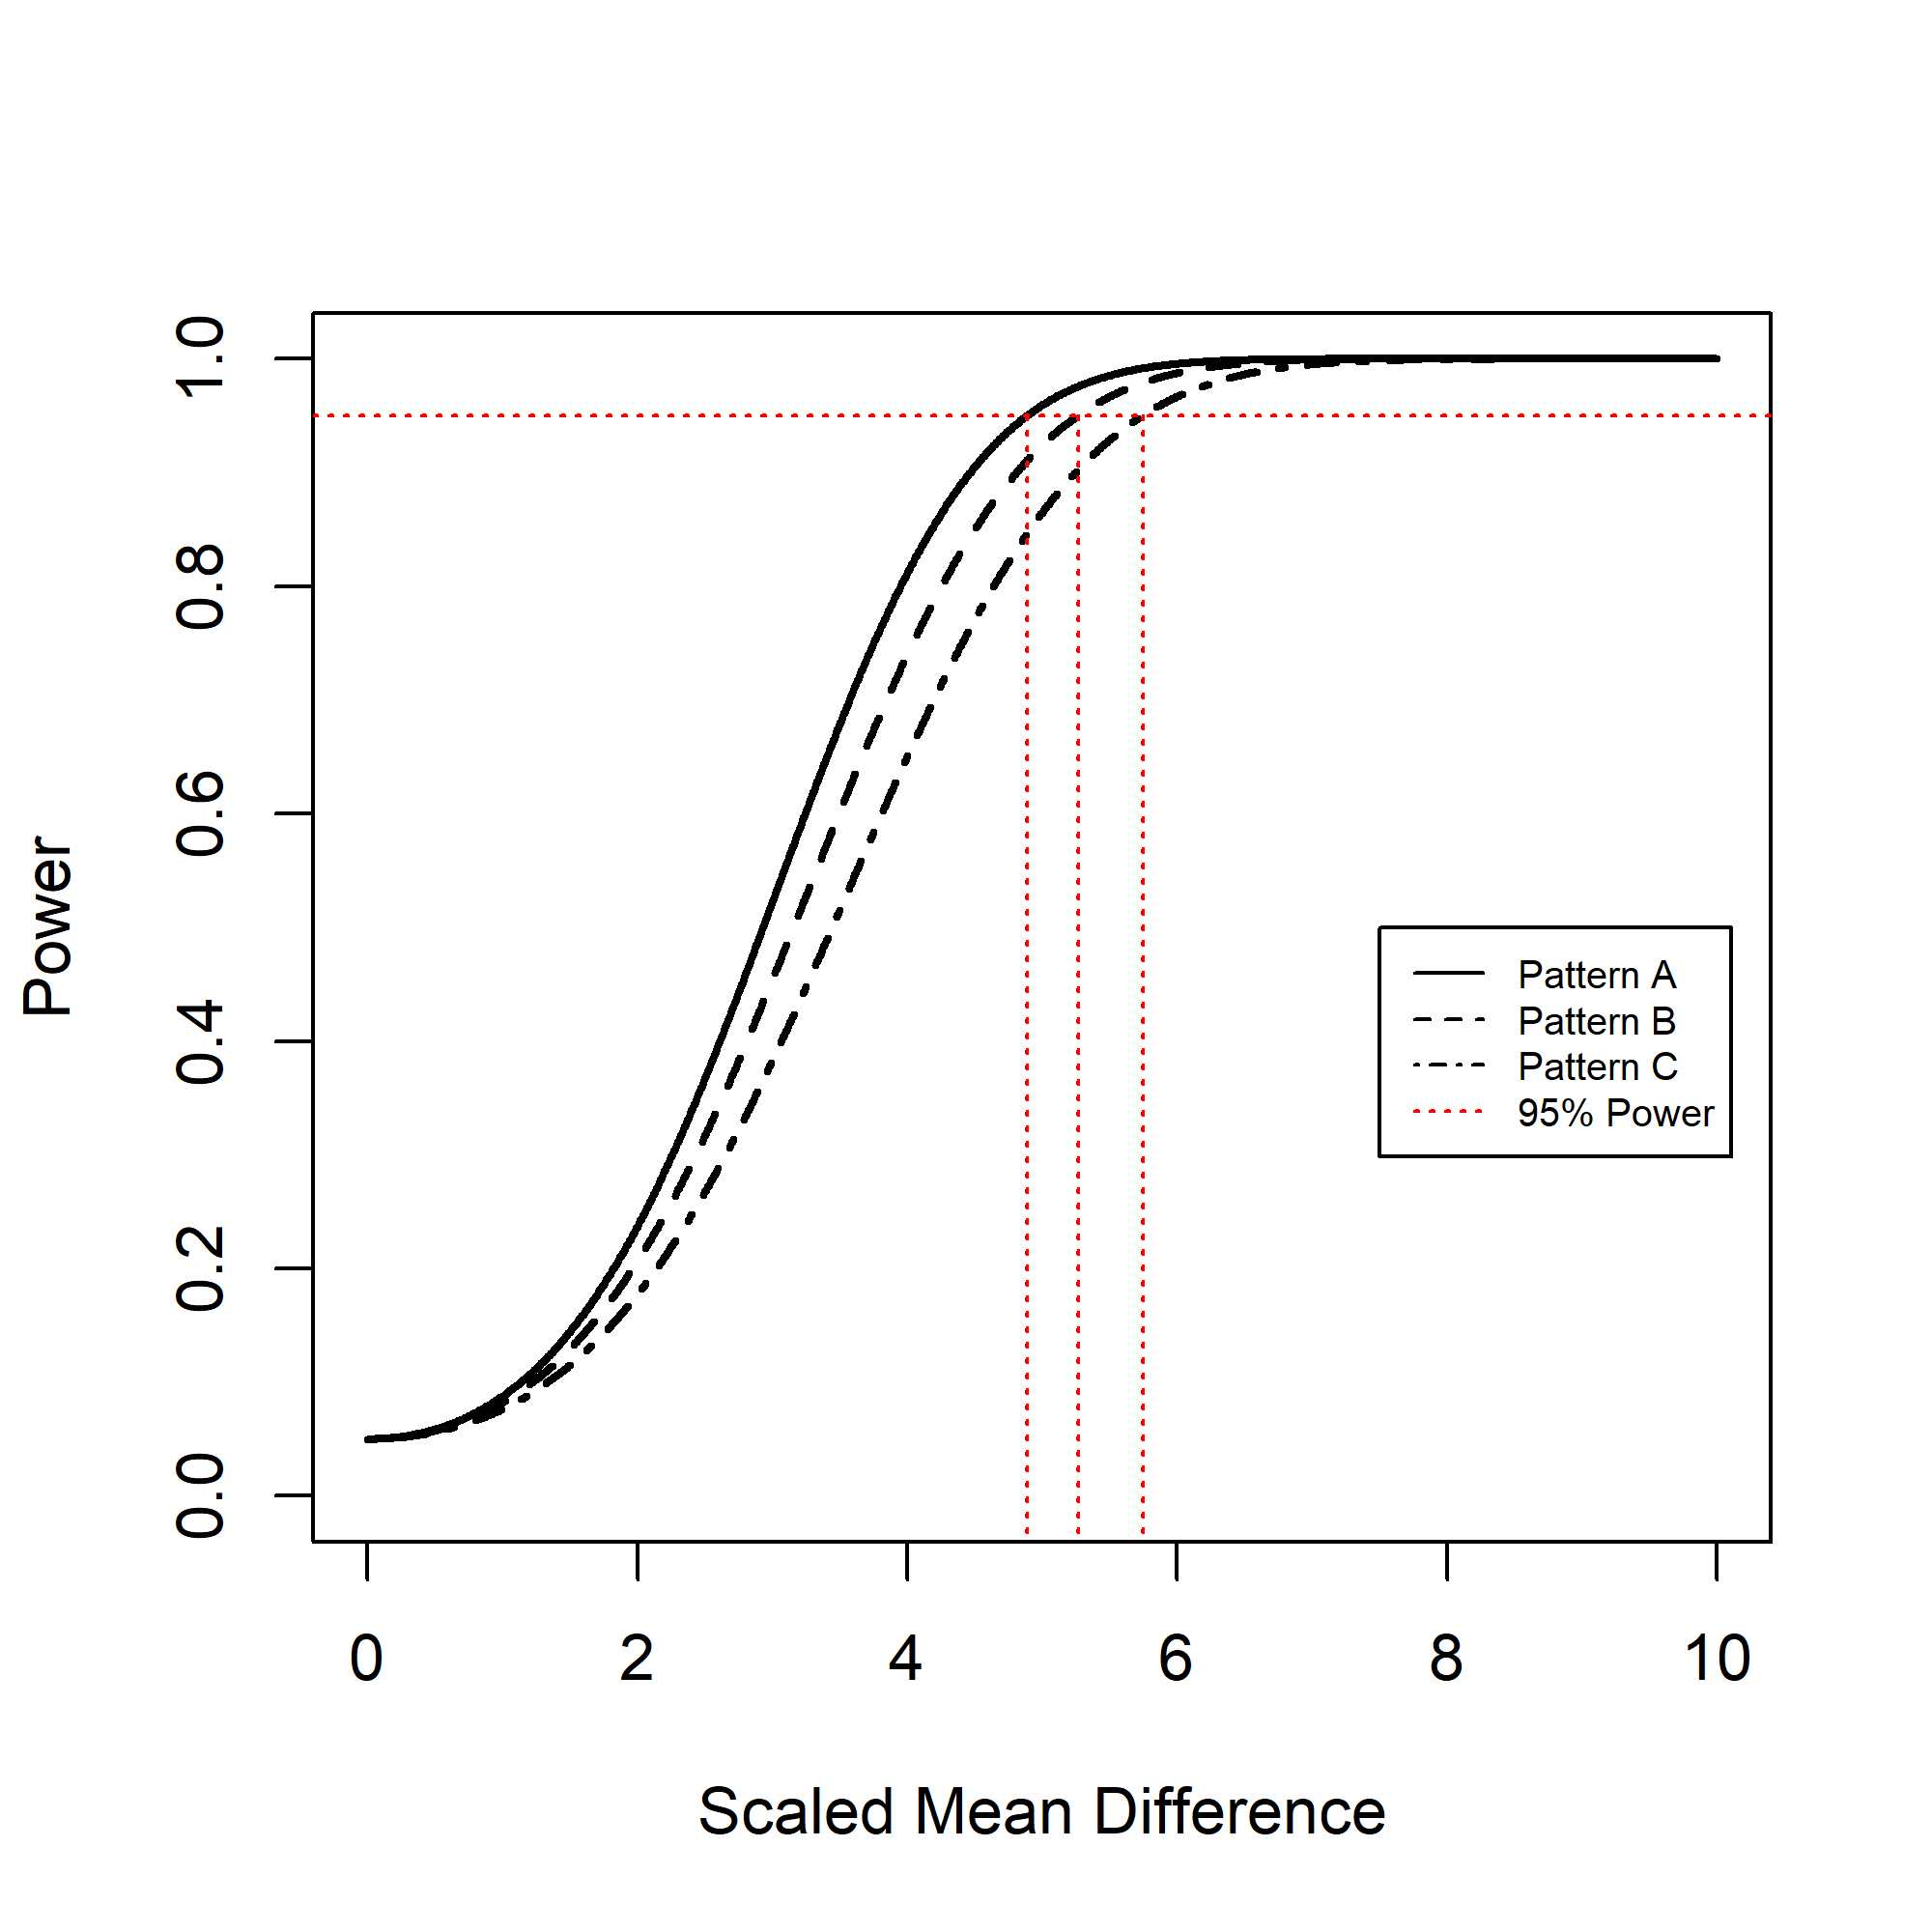
\includegraphics{figure_3}
\caption{Power for a randomized controlled trial}\label{horse}
\end{figure}

\end{document}
